\section{Vorlesung 10: Modellierung von Objektverhalten}

In den bisherigen Vorlesungen haben wir das Verhalten 
\marginline{Modellierung von Verhalten mit UML}
von Systemen und Prozessen mit Petrinetzen modelliert. In dieser und auch in der nächsten Vorlesung werden wir uns ansehen, welche Modellierungsmöglichkeiten die UML -- die ja explizit für die objektorientierte Softwareentwicklung geschaffen wurde -- für die Ver\-haltens\-model\-lierung anbietet. Dabei interessiert uns auch, welche Bezüge es zwischen diesen Diagrammen der UML und Petrinetz-Modellen gibt und an welchen Stellen man die Ihnen bekannten Prozesse, Abläufe, Aktivitäten, Aktionen etc. in den UML-Diagrammen findet.

Wir betrachten in dieser Vorlesung zunächst die Modellierung von \textbf{Objektverhalten} mithilfe der UML-Diagrammarten \textit{Zustandsdiagramm} und \textit{Sequenzdiagramm}. Vorlesung 11 wird dann mit dem UML-Aktivitätsdiagramm zurückkehren auf die Ebene der Modellierung von (Realwelt)-Prozessen.

Wir beginnen mit einem Beispiel aus dem Zookontext. Wir möchten das Verhalten eines Zoofahrzeugs modellieren, das das benötigte Futter zu den Gehegen der Tiere transportiert und beschreiben sein (mögliches) Verhalten folgendermaßen:

\vspace{2mm} %%% für Druck

\begin{addmargin}[25pt]{25pt}
	Das Fahrzeug 
	\marginline{Beispiel Zoo}
	soll seinen Standort zwischen seiner Garage und dem Futterlager wechseln können. Zudem muss es, wenn das Benzin knapp wird, an die Tankstelle fahren und wieder aufgetankt werden. Wenn sich das Zoofahrzeug am Futterlager befindet, kann es beladen werden -- abhängig davon, zu welchen Gehegen es danach fahren soll, wird es mit unterschiedlichem Futter beladen -- und fährt dann in beladenem Zustand zu seinen Zielen (z.B. Löwengehege oder Affengehege). Nach Erledigung seiner Auslieferungen kann es zurück in seine Garage fahren, zurück zum Lager, falls weiteres Futter geladen werden muss, oder auch zur Tankstelle, falls notwendig.
\end{addmargin}

\vspace{2mm} %%% für Druck

Das Verhalten des Zoofahrzeugs könnte man mit Petrinetzen abbilden, 
\marginline{Modellierung des Beispiels mit Petrinetzen}
indem man die lokalen Zustände („Tank leer“, „Tank halbvoll“, „Standort Affengehege“, „Standort Tankstelle“, „Fahrzeug mit Löwenfutter beladen“ ...) des Objekts „Fahrzeug“ durch Stellen modelliert, über die Markenverteilung auf einer Stelle dann die möglichen Objektzustände (Kombination der Wertebelegung aller Attribute des Objekts) abbildet und über die Transitionen die möglichen Änderungen der Objektzustände vorsieht. In der Videovorlesung wird ein solches Petrinetz gezeigt und erklärt.

Im objektorientierten Softwareengineering verwendet man für die Darstellung von Objektverhalten häufig das UML-Zustandsdiagramm.

\subsection*{UML-Zustandsdiagramm}

Zustandsdiagramme gehören zu den Verhaltensdiagrammen der UML. Sie basieren auf den sogenannten State Charts von David Harel \cite{har87}, wobei die Semantik allerdings etwas verändert wurde. Zustandsdiagramme werden in Softwareentwicklungsprojekten sowohl in der Anforderungsermittlung/-analyse eingesetzt -- hier meist zur Diskussion über mögliche Zustände und Verhalten von Realwelt-Objekten -- als auch im Zuge des Entwurfs des Softwareprodukts. Im letzteren Fall wird mit den Diagrammen insbesondere das gewünschte Verhalten späterer Software-Objekte spezifiziert. In beiden Fällen werden Zustandsdiagramme in der Regel in Kombination mit Klassendiagrammen verwendet, aus denen sich der Kontext ergibt, in dem das betrachtete Objekt operiert. Im Unterschied zu den Aktivitätsdiagrammen (s. Vorlesung 11), die auch Verhaltensdiagramme sind und die Aktivitäten eines Systems betrachten, konzentrieren sich Zustandsdiagramme auf die \textit{Reaktionen} von Systemelementen: in welcher Weise soll das betrachtete Objekt auf das Eintreten bestimmter Ereignisse reagieren?

Kehren wir zum Zoofahrzeug zurück und betrachten es als Objekt. Seine Zustände bedingen das mögliche Verhalten des Fahrzeugs. Schon bei solch einer noch wenig komplexen Beschreibung von Objektverhalten müssen wir für die Zustände, die das Objekt "`Zoofahrzeug"' annehmen kann, mehrere Attribute vorsehen, zum Beispiel „Füllstand des Tanks“, „Standort“, „Ladung“. Wenn wir alle möglichen Zustände (alle möglichen Kombinationen der Wertebelegungen aller Attribute) und sämtliches von diesen Zuständen abhängige mögliche Verhalten einzeln modellieren wollten, würde ein Diagramm sehr schnell unübersichtlich werden bzw. praktisch gar nicht erstellbar sein. 

Das UML-Zustandsdiagramm 
\marginline{Modellierung des Beispiels mit UML-Zustands\-diagrammen}
abstrahiert daher von den konkreten Zuständen eines Objekts und fasst mehrere Objektzustände zu einem Konstrukt (Zustand genannt!) zusammen. Also Vorsicht: ein Zustand in einem UML-Zustandsdiagramm ist in den meisten Fällen nicht gleichbedeutend mit genau einem Objektzustand, sondern umfasst eine Menge von Zuständen dieses Objekts. Zu einem Diagramm-Zustand zusammenfassen kann man alle Objektzustände, die ähnliches Verhalten zeigen, d.h. die auf gleiche Ereignisse in gleicher Weise reagieren. Zum Beispiel werden vermutlich alle Objektzustände, die mit einem halb vollen Tank des Zoofahrzeugs und alle, die mit einem dreiviertel vollen Tank zu tun haben, bezüglich ihres Verhaltens sehr ähnlich sein. 

\vspace{\baselineskip} %%% für Druck

\begin{figure}[!htbp]
	\centering
	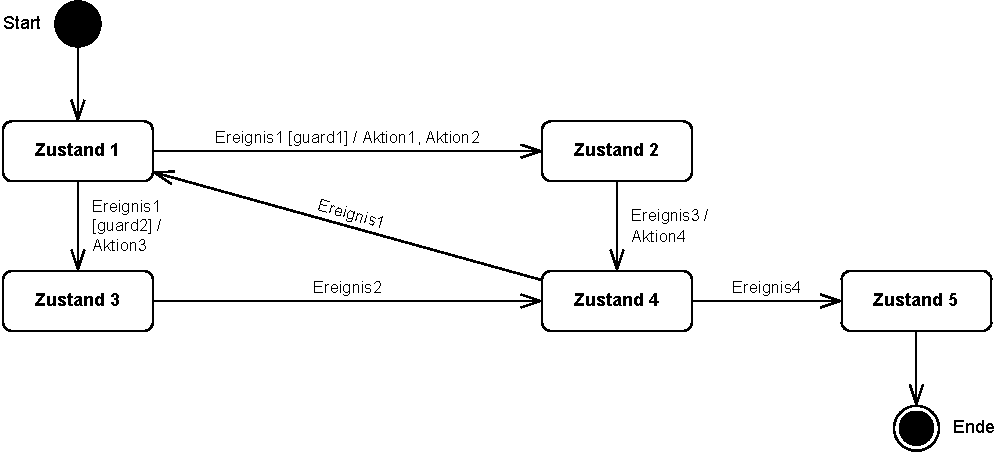
\includegraphics[scale=0.7]{Bilder/Kapitel-5/uml_zustandsdiagramm.pdf}
	\caption{Grundlegende Elemente eines UML-Zustandsdiagramms}
	\label{fig:uml_zustandsdiagramm}
\end{figure}

\vspace{\baselineskip} %%% für Druck

Abbildung~\ref{fig:uml_zustandsdiagramm} zeigt die wichtigsten Elemente eines UML-Zustandsdiagramms. 
\marginline{Zustände}
Die \textit{Zustände} werden mit abgerundeten Rechtecken modelliert. Das modellierte Objekt befindet sich immer in genau einem Zustand -- in Petrinetz-Terminologie gedacht: es gibt genau eine Marke und diese befindet sich in dem Zustand, in dem das Objekt gerade ist. Die gerichteten Pfeile modellieren die Übergänge zwischen den Zuständen, sie heißen \textit{Transitionen}.
\marginline{Transitionen}
Der Übergang von einem Zustand in einen anderen wird ausgelöst durch ein \textit{Ereignis}. Das auslösende Ereignis wird als Beschriftung an die Transition notiert. Die UML unterscheidet verschiedene Formen von Ereignissen. Die wichtigsten sind das \textit{Call Event} (Anfrage) -- dieses findet man häufig in Form von Operationsaufrufen in Zustandsdiagrammen, die im Rahmen des Entwurfsprozesses erstellt werden -- das \textit{Signal Event} (asynchrones Signal), das \textit{Time Event} (Abhängigkeit von Zeit) und das \textit{Change Event} (Bedingung).

\vspace{0.9mm} %%% für Druck

Wenn ein Ereignis eintritt, 
\marginline{Ereignis} 
wechselt das Objekt in den durch die entsprechende Transition definierten Folgezustand. „Auf diesem Weg“ können zudem Aktivitäten stattfinden, und zwar sowohl Aktivitäten, 
\marginline{Aktivitäten}
die durch das Objekt selber durchgeführt werden, als auch Aktivitäten anderer Objekte im umgebenden System. In letzterem Fall kann ein Zustandsdiagramm ohne Kenntnis des Kontextes (z.B. durch vorliegende andere UML-Diagramme) für die Leser aber schnell unverständlich werden. Aktivitäten werden im Zustandsdiagramm ebenfalls an den Transitionen notiert, vom Ereignis jeweils getrennt durch einen Schrägstrich („/“). 

\vspace{0.9mm} %%% für Druck

Dasselbe Ereignis kann durchaus mehrfach im Zustandsdiagramm vorkommen. Je nachdem, von welchem Zustand die zugehörige Transition ausgeht, wird es aber unterschiedliches Verhalten des Objekts auslösen. Zum Beispiel könnte das Zeitereignis „Mittagszeit“ dafür sorgen, dass das Zoofahrzeug zum Löwengehege fährt, sofern es Löwenfutter geladen hat. Hat es dagegen Affenfutter geladen, sollte dasselbe Ereignis dazu führen, dass es zum Affengehege fährt. Hat das Fahrzeug Affenfutter geladen und gleichzeitig kaum noch Benzin im Tank, wird es wieder ein anderes Verhalten zeigen und vor der Fahrt zum Affengehege noch die Tankstelle aufsuchen.

\vspace{0.9mm} %%% für Druck

Man kann Zustandsdiagramme mit einem Startzustand 
\marginline{Start- und Endzustände}
und einem oder mehreren Endzuständen ausstatten. Ein schwarz ausgefüllter Kreis kennzeichnet den Startzustand, ein weißer Kreis mit schwarzem Punkt -- der leider so aussieht wie bei Petrinetzen ein lokaler Startzustand -- einen Endzustand.

\vspace{0.9mm} %%% für Druck

In Zustandsdiagrammen ist Nichtdeterminismus ein Fehlerfall, 
\marginline{Nicht\-determinismus}
eine Konstruktion wie in Abbildung~\ref{fig:zustandsdiagramme} oben darf daher nicht vorkommen. Hier ist nicht eindeutig festgelegt, in welchen der drei Zustände das Objekt wechseln soll, wenn das Ereignis „Mittagszeit“ eintritt. Die gängigste Variante eine solche Situation deterministisch zu modellieren, ist die Verwendung von \textit{Guards}.
\marginline{Guard}
Abbildung~\ref{fig:zustandsdiagramme} unten zeigt diese Lösung. Der Guard, eine Bedingung, die sich zum Beispiel auf einen Attributwert des Objekts beziehen kann, wird in eckigen Klammern hinter das Ereignis geschrieben. Die verschiedenen Guards an den Transitionen müssen so formuliert werden, dass immer nur höchstens einer der Guards desselben Ereignisses zutrifft. Es sollte auch nicht der Fall eintreten, dass keiner der Guards zutrifft; das wäre zwar nach Diagramm-Regeln nicht verboten, macht semantisch aber keinen Sinn. 


\begin{figure}[t]
	\vspace{5mm} %%% für Druck
	\centering
	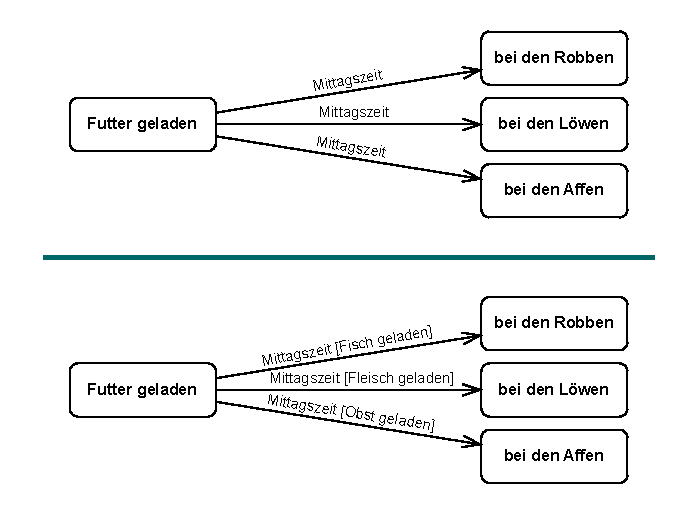
\includegraphics[scale=1.0]{Bilder/Kapitel-5/zustandsdiagramme.pdf}
	\caption[Ein fehlerhaftes nichtdeterministisches und ein korrektes deterministisches Zustandsdiagramm]{Ein fehlerhaftes nichtdeterministisches (oben) und ein korrektes deter\-ministisches (unten) Zustandsdiagramm}
	\label{fig:zustandsdiagramme}
	\vspace{\baselineskip} %%% für Druck
\end{figure}


\vspace{0.9mm} %%% für Druck

Neben den vorgestellten Grundelementen bietet die UML für Zustandsdiagramme einige weitere Elemente an, mit denen man Verhalten detaillierter spezifizieren kann. Darunter sind auch Möglichkeiten Verzweigungen und Schleifen zu modellieren, die man häufig benötigt, wenn Zustandsdiagramme (für Software-Objekte) schon sehr implementierungsnah sein sollen. Bei Diagrammen mit sehr vielen modellierten Zuständen lohnt sich zudem der Einsatz des Elements „zusammengesetzter Zustand“ (wird in der Videovorlesung an einem Beispiel gezeigt), mit dem man Hierarchien von Zuständen darstellen kann.

\subsection*{UML-Sequenzdiagramm}

Auch mit den UML-Sequenzdiagrammen modelliert man Verhalten, aber nicht nur das Verhalten eines einzelnen Objekts, sondern vor allem die Kommunikation (Austausch von Nachrichten) zwischen Objekten. 

Sequenzdiagramme haben ihren Ursprung in den Message Sequence Charts aus dem Telekommunikationsbereich, auch wenn der Blick dort nicht auf Objekte, sondern auf größere Einheiten gerichtet war. Im Softwareengineering kann man Sequenzdiagramme während der Anforderungsermittlung einsetzen, um Nachrichtenflüsse zwischen Personen oder Systemkomponenten in Geschäftsprozessen, die das spätere Softwareprodukt unterstützen soll, deutlich zu machen. Wesentlich häufiger werden Sequenzdiagramme aber beim Entwurf eingesetzt und sind schon sehr implementierungsnah. Auch die Reaktion des Softwareystems auf die Bedienung der GUI durch den Nutzer (was genau passiert, wenn der Nutzer diesen Button klickt, dieses Menü öffnet etc.) ist ein typischer Einsatzzweck eines Sequenzdiagramms.

Kehren wir kurz nochmal zu den Petrinetzen zurück und überlegen, wie wir Objektkommunikation mit Petrinetzen modellieren würden.

\pagebreak %%% für Druck

\begin{figure}[!htbp]
	\vspace{5mm} %%% für Druck
	\centering
	\begin{tabular}{ll}
		%--------------------------------------
		% \hline
		% 1. Reihe
		\textbf{Objekte} & 
		\parbox{0.75\textwidth}{
			\scalebox{0.6}{
				\petrinetz{
					\draw[colDummyLine, very thick] (-0.5, -1) rectangle (16.5, 1);
					
					% Places
					\node[place, tokens=1, label=above:$s_2$] (s2) at ( 6,  2) {}; 
					\node[place, tokens=0, label=below:$s_4$] (s4) at ( 6, -2) {}; 
					\node[place, tokens=0, label=right:$s_3$] (s3) at (10,  0) {}; 
					
					% Transitions
					\node[transition, label=left: $t_2$] (t2) at (4,  0) {}; 
					\node[transition, label=above:$t_3$] (t3) at (8,  2) {}; 
					\node[transition, label=below:$t_5$] (t5) at (8,  0) {};
					\node[transition, label=below:$t_4$] (t4) at (8, -2) {};
					
					%Edges
					\draw 
					(t2) edge[post, bend left=30] (s2) 
					(s2) edge[post] (t3) 
					(t3) edge[post, bend left=30] (s3) 
					(s3) edge[post] (t5) 
					(s3) edge[post, bend left=30] (t4) 
					(t4) edge[post] (s4) 
					(t5) edge[post, bend left=30] (s2) 
					(s4) edge[post, bend left=30] (t2)
					;
					
					%					\draw (s2) edge[post] (t3);
					%					\draw (t3) edge[post] (s3);
					%					\draw (s3) edge[post] (t4);
					%					\draw (t4) edge[post] (s4);
					%					\draw (s4) edge[post] (t2);
					%					\draw (t2) edge[post] (s2);
					%					\draw (s3) edge[post] (t5);
					%					\draw (t5) edge[post] (s2);
				}
			}
		}
		\\
		%--------------------------------------
		%--------------------------------------
		% \hline
		&  \\ % eine Leerzeile für den Abstand
		&  \\ % eine Leerzeile für den Abstand
		&  \\ % eine Leerzeile für den Abstand
		%--------------------------------------
		% \hline
		% 2. Reihe
		\textbf{Ablauf} & 
		\parbox{0.75\textwidth}{
			\scalebox{0.6}{
				\petrinetz{
					\draw[colDummyLine](-0.5, 0) -- (16.5, 0);
					
					% Places
					\node[place, tokens=1, label=above:$s_2$] (place2_1) at ( 0, 0) {};
					\node[place, tokens=0, label=above:$s_3$] (place3_1) at ( 4, 0) {};
					\node[place, tokens=0, label=above:$s_2$] (place2_2) at ( 8, 0) {};
					\node[place, tokens=0, label=above:$s_3$] (place3_2) at (12, 0) {};
					\node[place, tokens=0, label=above:$s_4$] (place4)   at (16, 0) {};
					
					% Transitions
					\node[transition, label=center:$t_3$] (trans3_1) at ( 2, 0) {};
					\node[transition, label=center:$t_5$] (trans5)   at ( 6, 0) {};
					\node[transition, label=center:$t_3$] (trans3_2) at (10, 0) {};
					\node[transition, label=center:$t_4$] (trans4)   at (14, 0) {};
					
					% Edges
					\draw (place2_1) edge[post] (trans3_1);
					\draw (trans3_1) edge[post] (place3_1);
					\draw (place3_1) edge[post] (trans5);
					\draw (trans5)   edge[post] (place2_2);
					\draw (place2_2) edge[post] (trans3_2);
					\draw (trans3_2) edge[post] (place3_2);
					\draw (place3_2) edge[post] (trans4);
					\draw (trans4)   edge[post] (place4);
				}
			}
		}
		\\
		%--------------------------------------
		%--------------------------------------
		% \hline
		&  \\ % eine Leerzeile für den Abstand
		&  \\ % eine Leerzeile für den Abstand
		&  \\ % eine Leerzeile für den Abstand
		%--------------------------------------
		% \hline
		% 3. Reihe
		\textbf{Kommunikation} & 
		\parbox{0.75\textwidth}{
			\scalebox{0.6}{
				\petrinetz{
					\draw[colDummyLine, very thick] (-0.5, -5) rectangle (16.5, 1);
					
					% Places
					\node[place, tokens=1] (s1) at (0,  0) {};
					\node[place, tokens=0] (s2) at (4,  0) {};
					\node[place, tokens=0] (s3) at (8,  0) {};
					\node[place, tokens=0] (s4) at (12, 0) {};
					\node[place, tokens=0] (s5) at (16, 0) {};
					
					\node[place, tokens=0] (s6) at (2,  -2) {};
					\node[place, tokens=0] (s7) at (10, -2) {};
					\node[place, tokens=0] (s8) at (12, -2) {};
					
					\node[place, tokens=1] (s9)  at (0,  -4) {};
					\node[place, tokens=0] (s10) at (4,  -4) {};
					\node[place, tokens=0] (s11) at (8,  -4) {};
					\node[place, tokens=0] (s12) at (12, -4) {};
					\node[place, tokens=0] (s13) at (16, -4) {};
					
					% Transitions
					\node[transition] (t1) at (2,  0) {};
					\node[transition] (t2) at (6,  0) {};
					\node[transition] (t3) at (10, 0) {};
					\node[transition] (t4) at (14, 0) {};
					
					\node[transition] (t5) at (2,  -4) {};
					\node[transition] (t6) at (6,  -4) {};
					\node[transition] (t7) at (10, -4) {};
					\node[transition] (t8) at (14, -4) {};
					
					% Edges
					% obere Reihe
					\draw (s1) edge[post] (t1);
					\draw (t1) edge[post] (s2);
					\draw (s2) edge[post] (t2);
					\draw (t2) edge[post] (s3);
					\draw (s3) edge[post] (t3);
					\draw (t3) edge[post] (s4);
					\draw (s4) edge[post] (t4);
					\draw (t4) edge[post] (s5);
					
					% untere Reihe
					\draw (s9)  edge[post] (t5);
					\draw (t5)  edge[post] (s10);
					\draw (s10) edge[post] (t6);
					\draw (t6)  edge[post] (s11);
					\draw (s11) edge[post] (t7);
					\draw (t7)  edge[post] (s12);
					\draw (s12) edge[post] (t8);
					\draw (t8)  edge[post] (s13);
					
					% dazwischen
					\draw (t1) edge[post] (s6);
					\draw (s6) edge[post] (t5);
					\draw (t3) edge[post] (s7);
					\draw (s7) edge[post] (t7);
					\draw (t7) edge[post] (s8);
					\draw (s8) edge[post] (t4);
				}
			}
		}
		\\
		%\hline
	\end{tabular}
	\vspace{\baselineskip} %%% für Druck
	\caption{Kommunikation zwischen Objekten in Petrinetz-Modellierung}
	\label{fig:kommunikation_zw_objekten}
\end{figure}


Abbildung~\ref{fig:kommunikation_zw_objekten} zeigt oben ein Petrinetz, mit dem wir das mögliche Verhalten von uns interessierenden Objekten modelliert haben. In der Mitte ist ein möglicher Ablauf für ein konkretes Objekt dargestellt. Dieser Ablauf ist rein sequentiell, weil das Objektverhalten keinerlei Nebenläufigkeit aufweist. Unten in der Abbildung sehen Sie Abläufe von zwei verschiedenen Objekten, wobei wir in der Abbildung nicht dargestellt haben, welche Transitionen genau geschaltet wurden (die zwei horizontalen Ketten aus unbeschrifteten Stellen und Transitionen). Die Kommunikation der beiden Objekte modellieren wir, indem wir ihre Abläufe an den Positionen, an denen Kommunikation stattfindet, über Stellen miteinander verbinden. Hier schicken sich die beiden Objekte Nachrichten (z.B. Operationsaufrufe). Bei der links dargestellten Kommunikation handelt es sich um eine \textit{asynchrone}, rechts um eine \textit{synchrone} Nachricht. 
\marginline{synchrone und asynchrone Kommunikation}
Bei asynchroner Kommunikation kann der Sender mit seiner Arbeit fortfahren, unabhängig davon, wann und ob der Empfänger antwortet. Bei synchroner Kommunikation geht das nicht, der Sender wartet so lange, bis er eine Antwort erhält. Sie sehen daher rechts in der Abbildung, dass die nächste Transition des oberen Ablaufs erst schalten kann, nachdem die Transition des unteren Ablaufs geschaltet hat. Wo keine Kommunikation stattfindet, können die Objekte unabhängig voneinander, also nebenläufig agieren.

\pagebreak %%% für Druck

Die Modellierung von Objektkommunikation durch UML-Sequenzdiagramme funktioniert sehr ähnlich. Abbildung~\ref{fig:uml_sequenzdiagramm} zeigt die grundlegenden Elemente eines 
\linebreak %%% für Druck
Sequenzdiagramms. 


\begin{figure}[!htbp]
	\centering
	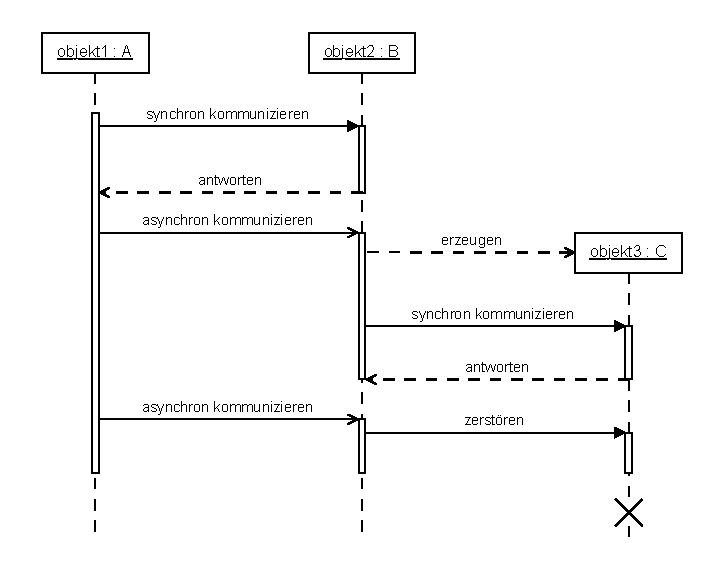
\includegraphics[scale=1.0]{Bilder/Kapitel-5/uml_sequenzdiagramm.pdf}
	\caption{Grundlegende Elemente eines UML-Sequenzdiagramms}
	\label{fig:uml_sequenzdiagramm}
\end{figure}


Statt von links nach rechts wie in unserer Petrinetz-Abbildung werden die Abläufe der Objekte von oben nach unten gezeichnet, symbolisiert durch die gestrichelten Linien, die man \textit{Lebenslinien} 
\marginline{Lebenslinie}
nennt. Die verschiedenen Objekte, die miteinander kommunizieren, sind dementsprechend horizontal nebeneinander angeordnet und werden wie im Klassendiagramm jeweils durch ein Rechteck dargestellt. Die Darstellung als anonymes Objekt einer Klasse geht auch. Zudem können auch menschliche Teilnehmer an der Interaktion modelliert werden (wie in anderen UML-Diagrammen als Strichmännchen). 

Sequenzdiagramme können durchaus die Kommunikation zwischen mehreren Objekten derselben Klasse modellieren. In der Regel interessiert aber die Kommunikation zwischen Objekten verschiedener Klassen. Man sieht sich im Sequenzdiagramm somit die Details genau der Beziehungen an, die man in Klassendiagrammen mit Assoziationen und Multiplizitäten modelliert hat.

Während mit der Lebenslinie im Sequenzdiagramm die komplette Lebenszeit eines Objekts symbolisiert wird, kennzeichnen die weißen Balken auf der Lebenslinie -- sie heißen \textit{Ausführungsbalken}
\marginline{Ausführungs\-balken}
-- die aktive Phase des Objekts. Synchrone und asynchrone Nachrichten werden durch unterschiedliche Pfeilspitzen dargestellt, die Antwort auf eine synchrone Nachricht durch einen gestrichelten Pfeil (s.~Abb.~\ref{fig:uml_sequenzdiagramm}). 

\pagebreak %%% für Druck

Zwei besondere Kommunikationsarten sind die Anforderung zur Erzeugung 
\marginline{Erzeugung und Zerstörung}
und zur Zerstörung eines Objekts. Die Erzeugungsanforderung, die dieselbe Pfeilart wie die Antwortnachricht hat, erkennt man daran, dass die Pfeilspitze nicht an einer Lebenslinie endet, sondern direkt an dem Objekt, das erzeugt wird. Die Zerstörungsanforderung gleicht syntaktisch einer synchronen Nachricht. Man erkennt sie -- neben der Tatsache, dass sie zumeist mit „zerstören“ beschriftet ist -- an dem großen {\Large$\times$} (ein sogenanntes Stopp-Symbol, das es in mehreren UML-Diagrammarten gibt) auf der Lebenslinie kurz unterhalb der eingehenden Nachricht.

Auch mit Sequenzdiagrammen kann man noch sehr viel detaillierter modellieren, zum Beispiel durch übereinanderliegende Ausführungsbalken parallele Tätigkeiten des Objekts vorsehen oder über sogenannte Zustandsinvarianten die Teilnahme eines Objekts an der Kommunikation von seinem aktuellen Zustand abhängig machen. Für viele Einsatzzwecke im Softwareengineering reichen die grundlegenden Elemente des Sequenzdiagramms aber aus.
